\documentclass[a4paper,UKenglish,cleveref,autoref]{lipics-v2019}

\usepackage[ruled, vlined]{algorithm2e}
\usepackage{tikz}
\usepackage{booktabs}
\usepackage{tabulary}
\usepackage{makecell}

\bibliographystyle{plainurl}

\usetikzlibrary{positioning,calc,shapes,matrix}
\tikzstyle{snode}=[circle,inner sep=0.5mm, minimum size=2.5mm,draw = black, fill=black]
\tikzstyle{node}=[circle,inner sep=0.5mm,minimum size=5.25mm,draw = black]

\newcommand{\tdcch}{CATCHUp}

\author{Ben Strasser}{Karlsruhe Institute of Technology, Germany}{academia@ben-strasser.net}{}{}
\author{Dorothea Wagner}{Karlsruhe Institute of Technology, Germany}{dorothea.wagner@kit.edu}{}{}
\author{Tim Zeitz}{Karlsruhe Institute of Technology, Germany}{tim.zeitz@kit.edu}{https://orcid.org/0000-0003-4746-3582}{}
\title{Space-efficient, Fast and Exact Routing in Time-dependent Road Networks}
\authorrunning{B. Strasser, D. Wagner, and T. Zeitz}
\Copyright{Ben Strasser, Dorothea Wagner, and Tim Zeitz}

\ccsdesc[500]{Theory of computation~Shortest paths}
\ccsdesc[300]{Mathematics of computing~Graph algorithms}
\ccsdesc[500]{Applied computing~Transportation}

\keywords{realistic road networks, time-dependent route planning, shortest paths}

\acknowledgements{We thank Lars Gottesb\"uren and Michael Hamann for fruitful discussions and feedback.
We also thank Marcel Radermacher for his input on approximation algorithms.}

\nolinenumbers

\EventEditors{Fabrizio Grandoni, Peter Sanders, and Grzegorz Herman}
\EventNoEds{3}
\EventLongTitle{28th Annual European Symposium on Algorithms (ESA 2020)}
\EventShortTitle{ESA 2020}
\EventAcronym{ESA}
\EventYear{2020}
\EventDate{September 7--9, 2020}
\EventLocation{Pisa, Italy (Virtual Conference)}
\EventLogo{}
\SeriesVolume{173}
\ArticleNo{76}

\begin{document}

\maketitle

\begin{abstract}
We study the problem of computing shortest paths in massive road networks with traffic predictions.
Incorporating traffic predictions into routing allows, for example, to avoid commuter traffic congestions.
Existing techniques follow a two-phase approach:
In a preprocessing step, an index is built.
The index depends on the road network and the traffic patterns but not on the path start and end.
The latter are the input of the query phase, in which shortest paths are computed.
All existing techniques have either large index size, slow query running times, or may compute suboptimal paths.
In this work, we introduce \tdcch{} (Customizable Approximated Time-dependent Contraction Hierarchies through Unpacking), the first algorithm that simultaneously achieves all three objectives.
The core idea of \tdcch{} is to store paths instead of travel times at shortcuts.
Shortcut travel times are derived lazily from the stored paths.
We perform an experimental study on a set of real world instances and compare our approach with state-of-the-art techniques.
Our approach achieves the fastest preprocessing, competitive query running times and up to 30 times smaller indexes than competing approaches.
\end{abstract}

\newpage

\section{Introduction}
Routing in road networks is a well-studied topic with a plethora of real world applications.
The core problem is to compute a fastest route between a source and a target.
The idealized problem can be formalized as the classic shortest path problem.
Streets are modeled as arcs.
Street intersections are modeled as nodes.
Travel times are modeled as scalar arc weights.
Unfortunately, this idealized view does not model certain important real world effects.
An important example are recurring commuter congestions.
In this paper, we consider an extended problem in which travel times are time-dependent.
The travel time of an arc is a function of the moment where a car enters the arc.
Figure~\ref{fig:tdgraph} depicts an example.

Computing shortest-paths using Dijkstra's \cite{d-ntpcg-59} algorithm is possible both in the classical and in the time-dependent setting.
However, for many applications, its running time is too large.
To achieve fast running times, a two-phase approach is used.
In the first phase, the \emph{preprocessing} phase, an index is constructed.
The index only depends on the road networks and the time-dependent arc weights.
In the second phase, the \emph{query} phase, shortest paths are computed utilizing this index.

\begin{figure}
\centering
\begin{tikzpicture}[]
  \node [snode] at (0, 0) (v1) {};
  \node [snode] at (1.5, 0.8) (v2) {};
  \node [snode] at (3.2, -0.5) (v3) {};
  \node [snode] at (3, 1) (v4) {};
  \node [snode] at (5, 1.2) (v5) {};
  \node [snode] at (5.3, 0.2) (v6) {};

  \node [] at (10.268, .2) (ttf) {\includegraphics[width=.5\columnwidth]{fig/ttf.pdf}};

  \draw [->] (v1) -- (v2);
  \node at (0.3, 0.5) {\includegraphics[width=6mm]{fig/ttf2_stripped.pdf}};
  \draw [->] (v2) -- (v3);
  \node at (2.5, 0.5) {\includegraphics[width=6mm]{fig/ttf5_stripped.pdf}};
  \draw [->] (v1) -- (v3) node[midway,below] {\includegraphics[width=6mm]{fig/ttf_stripped.pdf}};
  \draw [<->] (v3) -- (v4) node[midway,right] {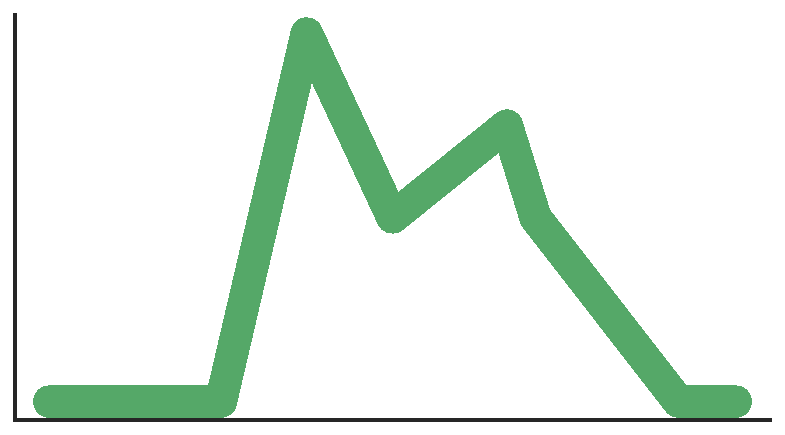
\includegraphics[width=6mm]{fig/ttf3_stripped.pdf}};
  \draw [<->] (v2) -- (v4) node[midway,above] {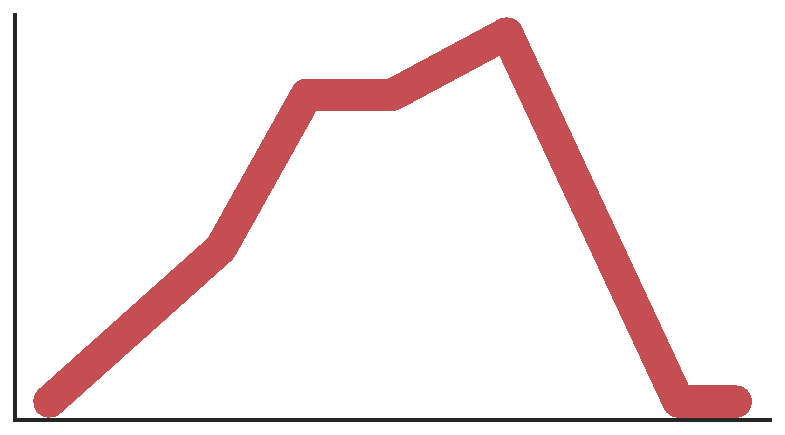
\includegraphics[width=6mm]{fig/ttf4_stripped.pdf}};
  \draw [->] (v4) -- (v5) node[midway,above] {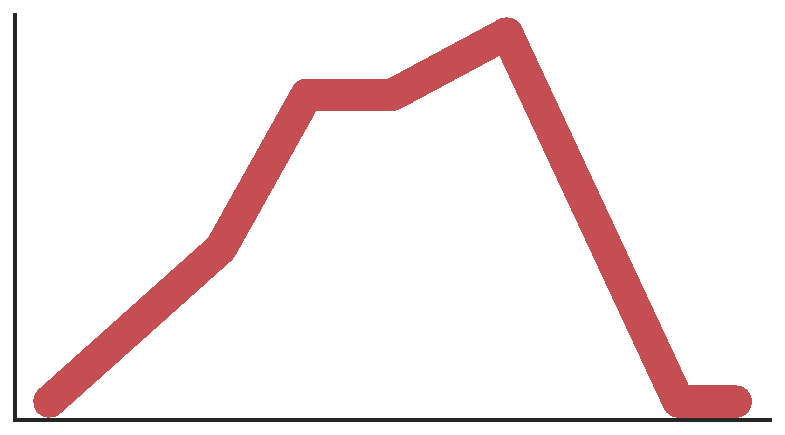
\includegraphics[width=6mm]{fig/ttf4_stripped.pdf}};
  \draw [->] (v5) -- (v6);
  \node at (5.6, .7) {\includegraphics[width=6mm]{fig/ttf_stripped.pdf}};
  \draw [<->] (v3) -- (v6) node[midway,below] {\includegraphics[width=6mm]{fig/ttf2_stripped.pdf}};

  \draw [-, dashed] (5.95, .87) -- (7.1, 1.4);
  \draw [-, dashed] (5.95, .53) -- (7.1, -.65);
\end{tikzpicture}
\caption{The graph of a small road network with predicted travel times for each road segment.}\label{fig:tdgraph}
\end{figure}

An important ingredient for many such two-phase techniques \cite{bdgmpsww-rptn-16,bd-sharc-09,dn-crdtd-12,dsw-cch-15,gssv-erlrn-12} are \emph{shortcuts}.
Shortcuts are additional arcs introduced during preprocessing, which bypass parts of the input graph like in Figure~\ref{fig:shortcut}.
The weight of a shortcut is set to the length of the shortest path between its endpoints.
When computing shortest paths, only few shortcuts are explored instead of many arcs in the input graph.
The path represented by a shortcut can be obtained lazily, for example by running local Dijkstra searches~\cite{dgpw-crprn-13}, or by iterating over possible middle nodes when shortcuts always represent exactly two other (shortcut) arcs~\cite{dsw-cch-15,gssv-erlrn-12}.

This approach has been extended to the time-dependent setting~\cite{bgsv-mtdtt-13,bdpw-dtdrp-16}.
Shortcuts are no longer associated with scalar weights.
Instead \emph{travel time functions} are used that map the entry time into a shortcut onto the travel time through it.
Unfortunately, in practice these functions become very complex.
Computing and storing them is expensive.
Implementations represent these functions typically as piecewise linear functions.
They are stored as a sequence of \emph{breakpoints}.
The number of breakpoints in a shortcut's function practically corresponds to the accumulated number of breakpoints of the functions of the arcs it bypasses.
Contrary to the classic setting, shortcuts aggregate the complexity of paths they represent, rather than skipping over it.
This leads to slow preprocessing and prohibitive memory consumption.

In this paper, we explore an alternative approach to shortcut travel time functions.
Rather than explicitly storing them and obtaining paths lazily, we store paths and obtain travel times lazily.
We expect that the shortest path between two nodes changes less frequently than the travel time.
Intuitively, going via a highway may be slower due to congestion but is usually still the fastest option.
Consider the functions $f$ and $g$ in Figure~\ref{fig:compression}.
These functions are travel time functions of two paths between the same endpoints and have many breakpoints.
If we want to store the travel time function of a shortcut between these endpoints, we need to store the function $h = \min(f, g)$.
Storing $h$ explicitly requires roughly a number of breakpoints proportional to the number of breakpoints in $f$ and $g$.
However, if we only store which path is the fastest, we only need to store the points in time when the faster path switches.
We expect significantly fewer switches than breakpoints.
In this paper, we employ this alternative approach to adapt an existing speed-up technique to the time-dependent setting, describe engineering techniques employed in our implementation, and present experimental results demonstrating that our approach significantly reduces memory consumption while achieving competitive query times.

\begin{figure}
\centering
\begin{subfigure}[b]{0.48\textwidth}
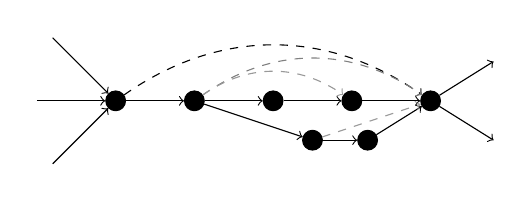
\begin{tikzpicture}[]
  \node [snode] at (1, 0) (v1) {};
  \node [snode] at (2, 0) (v2) {};
  \node [snode] at (3, 0) (v4) {};
  \node [snode] at (4, 0) (v5) {};
  \node [snode] at (5, 0) (v6) {};
  \node [snode] at (3.5, -0.5) (v7) {};
  \node [snode] at (4.2, -0.5) (v8) {};

  \draw [->] (.2,.8) -- (v1);
  \draw [->] (0,0) -- (v1);
  \draw [->] (.2,-.8) -- (v1);

  \draw [->] (v1) -- (v2);
  \draw [->] (v2) -- (v4);
  \draw [->] (v4) -- (v5);
  \draw [->] (v5) -- (v6);

  \draw [->] (v2) -- (v7);
  \draw [->] (v7) -- (v8);
  \draw [->] (v8) -- (v6);

  \draw [->] (v6) -- (5.8, .5);
  \draw [->] (v6) -- (5.8, -.5);

  \draw [->, dashed] (v1) to [bend left=35] (v6);
  \draw [->, dashed, draw=black!50] (v2) to [bend left=35] (v6);
  \draw [->, dashed, draw=black!40] (v2) to [bend left=35] (v5);
  \draw [->, dashed, draw=black!40] (v7) to (v6);

  \node at (0,-1) {};
\end{tikzpicture}
\caption{A shortcut arc (dashed, black) bypassing several nodes. In our implementation, shortcuts always skip over exactly one node and two arcs, which may in turn be shortcut arcs (dashed gray arcs).}\label{fig:shortcut}
\end{subfigure}
\hspace{1mm}
\begin{subfigure}[b]{0.48\textwidth}
\includegraphics[width=\textwidth]{fig/merge}
\caption{Travel time functions for two different paths between the same start and end node.}\label{fig:compression}
\end{subfigure}
\caption{Shortcuts and their travel time functions.}
\end{figure}

\subparagraph*{Related Work}

Routing in road networks has been extensively studied in the past decade.
An overview over the field can be found in \cite{bdgmpsww-rptn-16}.
Here, we focus on speed-up techniques for time-dependent road networks.
Several time-independent speed-up techniques have been generalized to the time-dependent setting.
ALT \cite{gh-cspas-05}, an approach using landmarks to obtain good A* \cite{hnr-afbhd-68} potentials has been generalized to TD-ALT \cite{ndls-bastd-12} and successively extended with node contraction to TD-CALT \cite{dn-crdtd-12}.
Even when combined with approximation, TD-CALT queries may take longer than 10\,ms on continental sized graphs.
SHARC \cite{bd-sharc-09}, a combination of ARC-Flags \cite{l-aefea-04} with shortcuts which allows unidirectional queries was also extended to the time-dependent scenario \cite{d-tdsr-11}.
It can additionally be combined with ALT yielding L-SHARC \cite{d-tdsr-11}.
SHARC can find short paths in less than a millisecond but does not always find a shortest path.
MLD/CRP \cite{dgpw-crprn-13,hsw-emlog-08} has been extended to TD-CRP \cite{bdpw-dtdrp-16} which can be used in a time-dependent setting.
TD-CRP requires approximation to achieve reasonable memory consumption.
It may find suboptimal paths.
Another approach is FLAT \cite{kmppwz-eotdr-16} and its extension CFLAT \cite{kppwz-iotdr-17a}.
CFLAT features sublinear query running time after subquadratic preprocessing and guarantees on the approximation error.
Unfortunately, preprocessing takes long in practice and generates a prohibitively large index size.

There are several approaches based on CH \cite{gssv-erlrn-12}.
Three were introduced in \cite{bgsv-mtdtt-13}: Time-dependent CH (TCH), inexact TCH, and Approximated TCH (ATCH).
TCH achieve great query performance but at the cost of a huge index size on state-of-the-art continental sized instances.
The index size can be reduced at the cost of exactness (inexact TCH) or query performance (ATCH).
An open-source reimplementation of \cite{bgsv-mtdtt-13} named KaTCH\footnote{\url{https://github.com/GVeitBatz/KaTCH}} exists.
A simple heuristic named Time-Dependent Sampling (TD-S) was introduced in \cite{s-dtdrr-17}.
It samples a fixed set of scalar values from the time-dependent functions.
It has manageable index sizes and fast query times but does not always find shortest paths.

\subparagraph*{Contribution and Outline}

In this work, we explore a variant of time-dependent CH, where shortcuts store paths instead of travel times.
We introduce \tdcch{} -- Customizable Approximated Time-dependent Contraction Hierarchies trough Unpacking, a time-dependent generalization of Customizable Contraction Hierarchies \cite{dsw-cch-15} and a thoroughly engineered implementation.
Preprocessing takes only a few minutes even on modern production-grade continental sized instances with tens of millions of nodes.
We also present algorithms which allow us to employ approximation to accelerate preprocessing without sacrificing exactness for the queries.
Our implementation achieves fast and exact queries with performance competitive to TCH queries while requiring up to 30 times less memory.

The rest of this paper is organized as follows.
In Section~\ref{sec:prelim}, we introduce some notation and existing algorithms we build on.
We describe our shortcut data structure, and the preprocessing and query algorithms in Section~\ref{sec:algos}.
In Section~\ref{sec:exp}, we discuss our experimental evaluation.
We conclude in Section~\ref{sec:conclusion}.

\section{Preliminaries}\label{sec:prelim}
We model road networks as directed graphs $G=(V,A)$.
A node $v \in V$ represents an intersection and an arc $a=uv \in A$ with $u,v \in V$ represents a road segment.
A path is a sequence of nodes $[v_1, ..., v_k]$ such that $v_i v_{i+1} \in A$.
Every arc $a$ has a \emph{travel time function} $f_a: \mathbb{R} \to \mathbb{R}^{>0}$ mapping departure time to travel time.
We assume that travel time functions fulfill the \emph{First-In-First-Out} (FIFO) property, that is for any $\sigma, \tau \in \mathbb{R}$ with $\sigma \leq \tau$, $\sigma + f(\sigma) \leq \tau + f(\tau)$ has to hold.
Informally, this means that it is not possible to arrive earlier by starting later.
If there are arcs that do not fulfill the FIFO property, the shortest path problem becomes $\mathcal{NP}$-hard~\cite{or-tnp-89}.
In our implementation, travel time functions are periodic piecewise linear functions represented by a sequence of \emph{breakpoints}.
We denote the number of breakpoints by $|f|$.

Given two travel time functions $f$ and $g$ for arcs $uv$ and $vw$, we are often interested in the travel time function of traversing first $uv$ and then $vw$, that is $(g \circ f)(\tau) = f(\tau) + g(f(\tau) + \tau)$.
Computing this function is called \emph{linking}.
When combining two travel time functions $f$ and $g$ for different paths $[u,...,v]$ with the same start and end, we often want to know the travel time of the best path between $u$ und $v$, that is $\min(f, g)$.
Computing this function is called \emph{merging}.
Both linking and merging can be implemented with coordinated linear sweeps over the breakpoints of both functions. % TODO explain linear sweep

Given a departure time $\tau$ and nodes $s$ and $t$, an earliest-arrival query asks for earliest point in time one can arrive at $t$ when starting from $s$ at $\tau$.
Such a query can be handled by Dijkstra's algorithm~\cite{d-ntpcg-59} with little modifications~\cite{d-aassp-69}.
The algorithm keeps track of the earliest known arrival time $\operatorname{ea}_v$ at each node $v$.
These labels are initialized with $\tau$ for $s$ and $\infty$ for all other nodes.
A priority queue is initialized with $(s,\tau)$.
In each step, the node $u$ with minimal earliest arrival $\operatorname{ea}_u$ is popped from the queue and outgoing arcs are \emph{relaxed}.
To relax an arc $uv$, the algorithm checks if $\operatorname{ea}_u + f_{uv}(\operatorname{ea}_u)$ improves $\operatorname{ea}_v$ and updates label and queue position of $v$ accordingly.
Once $t$ is extracted from the queue, the earliest arrival at $t$ is known.
To retrieve the shortest path, one can use \emph{parent pointers} which for each node store the previous node on the shortest path from $s$.
We refer to this algorithm as \emph{TD-Dijkstra}.

The \emph{A* algorithm} \cite{hnr-afbhd-68} is an extension to Dijkstra's algorithm.
It reduces the number of explored nodes by guiding the search towards $t$.
Each node $u$ has a potential $\rho_t(u)$ which is an estimate of the distance to $t$.
The priority queue is then ordered by $\operatorname{ea}_u + \rho_t(u)$.

\emph{Contraction Hierarchies}~(CH)~\cite{gssv-erlrn-12} is a speed-up technique exploiting the inherent hierarchy in road networks.
Nodes are heuristically ranked by their importance.
Nodes with higher rank should cover more shortest paths.
During preprocessing, all nodes are \emph{contracted} in order of ascending importance.
Contracting a node $v$ means removing it from the network but preserving all shortest distances among the remaining higher ranked nodes.
This is achieved by inserting \emph{shortcut arcs} between the neighbors of $v$ if a shortest path goes through $v$.
A shortcut is only necessary if it represents the only shortest path between its endpoints.
This can be checked with a local Dijkstra search (called \emph{witness search}) between the endpoints.
The result of the preprocessing is called an \emph{augmented graph}.
Queries can be answered by performing a bidirectional Dijkstra search on the augmented graph where only arcs to higher ranked nodes are relaxed.
The construction guarantees that this algorithm will find a shortest up-down-path which has the same length as shortest paths in the original graph.

\emph{Customizable Contraction Hierarchies}~(CCH)~\cite{dsw-cch-15} is a CH extension, splitting CH preprocessing into two steps where only the second one uses arc weights.
In the first step, a separator decomposition and an associated nested dissection order \cite{bcrw-s-16,g-ndrfe-73} are computed.
This order determines the node ranks.
Nodes in the top-level separators have the highest ranks, followed by the nodes of each cell, recursively ordered by the same method.
Then, nodes are contracted without running witness searches, so all potential shortcuts are added.
In the second step (called \emph{customization}), shortcut arc weights are computed.
All arcs are processed in ascending order of their lower ranked endpoint.
To process an arc $uv$, all \emph{lower triangles} $[u,w,v]$, where $w$ has lower rank than $u$ and $v$ are enumerated, checking if the path $[u,w,v]$ can improve the weight of $uv$.
The CH query algorithm can be reused without modifications.
Another query algorithm is described in~\cite{dsw-cch-15} based on the \emph{elimination tree} which does not need priority queues.
The parent of each node in the elimination tree is its lowest-ranked upward neighbor in the augmented undirected graph.
A nodes ancestors in the elimination tree are exactly the set of nodes that are reachable in a CH search from this node~\cite{bcrw-s-16}.
Thus, instead of exploring the search space through Dijkstra searches, the elimination tree query traverses the same nodes by traversing the path to the root in the elimination tree.

\section{Algorithms}\label{sec:algos}

In this section, we describe our algorithms, data structures and implementation.
Our approach builds upon CCH.
However, instead of storing travel time functions at shortcuts, we store unpacking information to efficiently reconstruct the represented paths in the original graph.
We start by describing our representation of this unpacking information.
Then, we continue by presenting our adapted CCH algorithms for the time-dependent setting.

\subsection{Shortcut Data Structure}\label{sec:shortcut}

The key element of our approach is the information we store with each shortcut.
We store time-dependent unpacking information, which allows us to efficiently reconstruct the original path represented by a shortcut for a point in time.
In (C)CH, shortcuts $uv$ are inserted when a node $w$ is contracted and the arcs $uw$ and $wv$ exist.
Thus, a shortcut $uv$ always skips over a triangle $[u,w,v]$.
However, there may be several triangles and which one is the fastest may change over time.
This is the information our shortcut data structure has to capture.

For each shortcut arc $uv$, we store a set of time-dependent \emph{expansions} $X_{uv}$ for unpacking.
See Figure~\ref{fig:shortcut_data} for an example.
For an expansion $x \in X_{uv}$, we denote the time during which $x$ represents the shortest path as the \emph{validity interval} $\Pi_x$ of $x$ and the lower node of the triangle $[u, w_x, v]$ as $w_x$.
In our implementation, the expansion information is represented as an array of triples $(\pi, u w_x, w_x v)$.
$\pi$ is the beginning of the validity interval and $uw$ and $wv$ are arc ids.
This information can be stored in 16 bytes for each entry -- 8 bytes for the timestamp and 4 bytes for each arc id.
Beside the unpacking information, we also store a scalar lower bound $\underline{b}_{uv}$ and an upper bound $\overline{b}_{uv}$ to prune unnecessary operations.

\begin{figure}
\centering
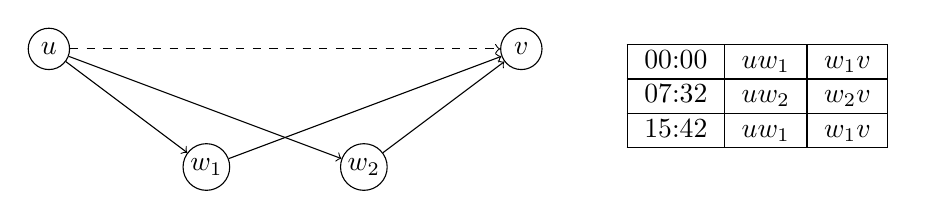
\begin{tikzpicture}[]
  \node [node] at (0, 0) (u) {$u$};
  \node [node] at (6, 0) (v) {$v$};
  \node [node] at (2, -1.5) (w1) {$w_1$};
  \node [node] at (4, -1.5) (w2) {$w_2$};

  \node at (9, -.6) {
    \begin{tabular}{|c|c|c|}
      \hline
      00:00 & $u w_1$ & $w_1 v$ \\
      \hline
      07:32 & $u w_2$ & $w_2 v$ \\
      \hline
      15:42 & $u w_1$ & $w_1 v$ \\
      \hline
    \end{tabular}
  };

  \draw [->, dashed] (u) -- (v);
  \draw [->] (u) -- (w1);
  \draw [->] (w1) -- (v);
  \draw [->] (u) -- (w2);
  \draw [->] (w2) -- (v);
\end{tikzpicture}
\caption{A shortcut with associated time-dependent unpacking information}\label{fig:shortcut_data}
\end{figure}

To obtain the shortest path represented by a shortcut $uv$ for a time $\tau$, we first need to determine the relevant expansion $x$ such that $\tau \in \Pi_x$.
This can be done performing a binary search in $X_{uv}$.
The shortcut can then be expanded to $[u,w_x,v]$.
However, $u w_x$ or $w_x v$ may also be shortcuts.
Thus, we recursively apply the operation to $(u, w_x)$ at $\tau$ and to $(w_x, v)$ at $\tau + f_{(u, w_x)}(\tau)$.
Evaluating the travel time of the first arc is always necessary to determine the time for unpacking for the second arc.
The travel time of a shortcut can be obtained by unpacking the path and then evaluating the travel times of the original arcs successively.

\subsection{Preprocessing}

The first step of CCH preprocessing is performed only on the topology of the graph.
Since no travel time functions are involved, we can adapt the algorithms of~\cite{dsw-cch-15} without modification.
We use InertialFlowCutter~\cite{ghuw-fbndocch-19} to obtain the nested dissection order.
To generate the shortcut augmented graph, we implement an improved contraction algorithm first presented in~\cite{z-cchtc-19}.
When contracting a node, we insert all upward neighbors of the current node only into the neighborhood of its lowest ranked upward neighbor.
This algorithm can be implemented to run in linear time in the size of the output graph.

The goal of the second step of preprocessing for classical CCH is to compute the shortcut weights.
So for our approach, we have to compute travel time bounds and unpacking information for all shortcuts\footnote{Note that actually all arcs in the augmented graph have to be treated as shortcuts. We represent arcs from the original graph as a special expansion element pointing to the original arc.}.
Recall that a shortcut $u v$ always bypasses one or many lower triangles $[u,w_i,v]$ for different nodes $w_i$, where $w_i$ has lower rank than $u$ and $v$.
For the bounds, we want to find the minimum and maximum travel time of the fastest travel time function between $u$ and $v$ over any $w_i$.
For the unpacking information, we need to determine for each point in time which triangle is the fastest.
Assuming we know the final travel time functions of all $u w_i$ and $w_i v$, we can obtain the travel time function for each triangle by linking $f_{u w_i}$ and $f_{w_i v}$.
By merging these linked functions, we can compute both the final bounds and the times during which each triangle is the fastest.
This leads to the following algorithmic schema:
Iterate over all arcs in a bottom-up fashion.
For each arc enumerate lower triangles.
Link and merge their functions to compute the function, bounds, and unpacking information of the current arc.
Keep the current arc's travel time function in memory until it is no longer needed.

We implement this schema as follows:
We process all arcs $u v$ ordered ascending by their lower ranked endpoint.
Since the middle node $w$ of a lower triangle $[u,w,v]$ has always lower rank than $u$ and $v$, the arcs $u w$ and $w v$ will have been processed already.
To process an arc $u v$ we enumerate lower triangles $[u,w,v]$.
For each triangle, we obtain the function of $[u,w,v]$ by linking the functions of the arcs $u w$ and $w v$, and merge it with the current function of the shortcut $u v$.
Once all arcs $u v$ have been processed where $u$ is the lower ranked endpoint, we drop the travel time functions of all arcs $w u$ where $u$ is the higher ranked endpoint.

When enumerating triangles, we order them ascending by $\underline{b}_{u w} + \underline{b}_{w v}$.
This way, we process triangles, which are likely faster first.
This gives us preliminary bounds on the travel time of $u v$.
Before linking the functions of another triangle $f_{u w}$ and $f_{w v}$, we check if $\overline{b}_{u v} \leq \underline{b}_{u w} + \underline{b}_{w v}$.
If so, the linked path would be dominated by the shortcut, and we can skip linking and merging completely.
If not, we link $f_{u w}$ and $f_{w v}$ and obtain $f_{[u,w,v]}$.
We still can skip merging if one function is strictly smaller than the other, that is either $\overline{b}_{u v} \leq \min(f_{[u,w,v]})$ or $\max(f_{[u,w,v]}) \leq \underline{b}_{u v}$.
Even if the bounds overlap, one function might still dominate the other.
To check for this case, we simultaneously sweep over the breakpoints of both functions, determining the value of the respectively other function by linear interpolation.
Only when this check fails, we perform the merge operation.

Before the time-dependent customization, we first use the basic and perfect customization algorithms from~\cite{dsw-cch-15} to compute preliminary scalar upper and lower bounds for all shortcuts.
With these bounds, we can skip additional linking and merging operations.
Also, we can remove some shortcuts completely, when a shorter path through higher ranked nodes exists.

\subparagraph*{Parallelization}

We employ both loop based and task based parallelism. % to distribute the workload of the customization among several cores.
The original CCH publication~\cite{dsw-cch-15} suggests processing shortcuts with their lower ranked endpoint on the same \emph{level} in parallel.
The level of a node is the level of its highest ranked downward neighbor increased by one, or zero if the node does not have downward neighbors.
We use this approach to process arcs in the top-level separators.

In~\cite{bsw-rttau-19}, a task based parallelism approach utilizing the separator decomposition of the graph is described.
Each task is responsible for a subgraph $G'$.
Removing the top-level separator in $G'$ decomposes the subgraph into two or more disconnected components.
For each component, a new task is spawned to process the shortcuts the component.
After all child tasks are completed, the shortcuts in the separator are processed utilizing the loop based parallelization schema.
If the size of subgraph $G'$ is below a certain threshold, the task processes the shortcuts in $G'$ sequentially without spawning subtasks.

\subparagraph*{Approximation}

As we process increasingly higher ranked shortcuts, the associated travel time functions become more and more complex.
This leads to two problems.
First, linking and merging becomes very time-consuming as running times scale with the complexity of the input functions.
Second, storing these functions for later reuse -- even though it is only temporary -- requires a lot of memory.
We employ approximation to mitigate these issues.
However, for exact queries, we need exact shortcut unpacking information.
We achieve this by lazily reconstructing parts of exact travel time functions during merging.

When approximating, we do not store one approximated function but two -- a lower bound function and an upper bound function with maximum error $\epsilon$ where $\epsilon$ is a configurable parameter.
These approximations replace the exact function stored for later merge operations and will also be dropped when no longer needed.
To obtain the bound functions, we first compute an approximation using the algorithm of Douglas and Peucker~\cite{dp-arnpr-73}.
Then, we add or subtract $\epsilon$ to the value of each breakpoint to obtain an upper or lower bound, respectively.
This yields valid upper or lower bounds, but they may not be as tight as possible.
Therefore, we iterate over all approximated points and move each point back towards the original function.
Both adjacent segments in the approximated functions have a minimum absolute error to the original function.
We move the breakpoint by the smaller of the two errors.
This yields sufficiently good bounds.

When linking approximated functions, we can link both lower and both upper bound functions.
Linking two lower bounds yields a valid lower bound function of the linked exact functions because of the FIFO property.
The same argument holds for upper bounds.

Merging approximated shortcuts is slightly more involved.
Our goal is to determine the exact unpacking information for each shortcut.
We use the approximated bounds to narrow down the time ranges where intersections are possible.
To identify these parts, we merge the first function's lower bound with the second function's upper bound and vice versa.
Where the bounds overlap, an intersection might occur.
We then obtain the exact functions in the overlapping parts through unpacking and perform the exact merging.
To obtain approximated upper and lower bounds of the merged function, we merge both lower bounds and both upper bounds.

We approximate whenever a function has more than $\beta$ breakpoints. % after merging.
This includes already approximated functions.
Both $\beta$ and the maximum error $\epsilon$ are tuning parameters which influence the performance (but not the correctness).

\subsection{Queries}

Our query algorithm is based on the CCH elimination tree query algorithm~\cite{dsw-cch-15}.
There are two challenges.
First, we can not perform a backwards search, as we do not know the arrival time at the target node.
Second, to evaluate the travel time of a shortcut, we need to obtain the path in the original graph.
Since unpacking shortcuts is expensive, we try to keep the number of these operations as small as possible.

Our query algorithm works in two phases.
In the first phase, we perform an elimination tree interval query using the lower and upper travel time bounds of the arcs.
The backward search is possible since these bounds are not time-dependent.
This yields a shortest path corridor.
This corridor is made up of both original and shortcut arcs and always contains the actual shortest path.
In the second phase, we perform a unidirectional Dijkstra search on this corridor, which lazily unpacks shortcuts.

\subparagraph*{Elimination Tree Interval Query}

The elimination tree interval query is a bidirectional search starting from both the source node $s$ and the target node $t$.
Node labels contain an upper $\overline{t}_v$ and a lower bound $\underline{t}_v$ on the travel time to/from the search origin and a parent pointer to the previous node.
The bounds $\overline{t}_s$, $\overline{t}_t$, $\underline{t}_s$, $\underline{t}_t$ are all initialized to zero in their respective direction, all other bounds to infinity.
We also track tentative travel time bounds for the total travel time from $s$ to $t$.
For both directions, the path from the start node to the root of the elimination tree is traversed.
For each node $u$, all arcs $u v$ to higher ranked neighbors are relaxed, that is checking if $\overline{t}_u + \overline{b}_{u v} < \overline{t}_v$ or $\underline{t}_u + \underline{b}_{u v} < \underline{t}_v$ and improving the bounds of $v$ if possible.
When the new travel time bounds from an arc relaxation overlap with the current bounds, more than one label has to be stored.
After both directions are finished, we have several meeting nodes in the intersection of the search spaces.
Where the sum of the forward and backward distance bounds of a node overlaps with the total travel time bounds, the parent pointers are traversed to the search origin and all arcs on the paths are marked as part of the shortest path corridor.

\subparagraph*{Lazy Corridor Dijkstra}

In the second query phase, we perform Dijkstra's algorithm on the corridor obtained in the first phase.
At the beginning, the corridor contains many shortcuts, which need to be unpacked, to determine their travel time.
We perform unpacking lazily.
The algorithm starts with the same initialization as a regular TD-Dijkstra.
All earliest arrivals are set to infinity, except for the start node which is set to the departure time.
The start node is inserted into the queue.
Then, nodes are popped from the queue until it is empty or the target node is reached.
For each node, all outgoing arcs within the shortest path corridor are relaxed.
When an arc is from the original graph, the travel time can be evaluated directly.
Shortcut arcs, however, need to be unpacked.
The unpacking algorithm defers the work as much as possible:
Only the first arc of the triangle of each shortcut will be recursively unpacked until an original arc is reached, the second arc will be added to the corridor.
See Figure~\ref{fig:lazy_unpack} for an example.
This way, we unpack only the necessary parts and avoid relaxing arcs multiple times when shortcuts share the same paths.

\begin{figure}
\centering
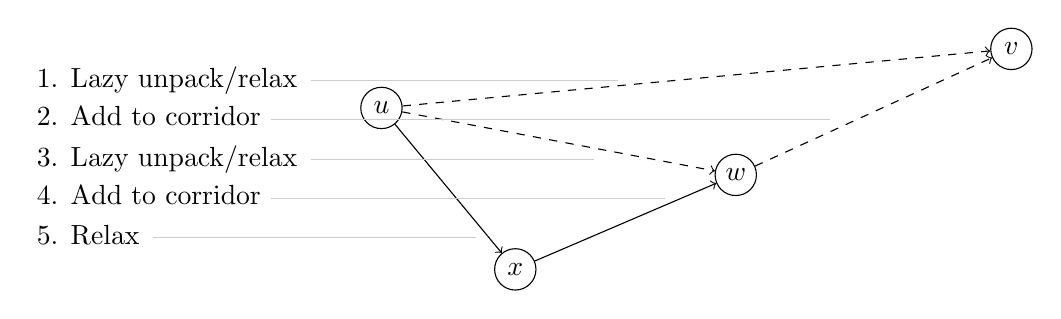
\begin{tikzpicture}[]
  \node [node] at (0, -.75)   (u) {$u$};
  \node [node] at (8, 0)      (v) {$v$};
  \node [node] at (4.5, -1.6) (w) {$w$};
  \node [node] at (1.7, -2.8) (x) {$x$};

  \draw [->, dashed] (u) to (v);
  \draw [->, dashed] (u) to (w);
  \draw [->, dashed] (w) to (v);
  \draw [->] (u) to (x);
  \draw [->] (x) to (w);

  \node [minimum width=1cm, minimum height=.5cm, anchor=north west] at (-4.5, .4 -.5)  (text_uv) {1. Lazy unpack/relax};
  \node [minimum width=1cm, minimum height=.5cm, anchor=north west] at (-4.5, .4 -1)   (text_wv) {2. Add to corridor};
  \node [minimum width=1cm, minimum height=.5cm, anchor=north west] at (-4.5, .4 -1.5) (text_uw) {3. Lazy unpack/relax};
  \node [minimum width=1cm, minimum height=.5cm, anchor=north west] at (-4.5, .4 -2)   (text_xw) {4. Add to corridor};
  \node [minimum width=1cm, minimum height=.5cm, anchor=north west] at (-4.5, .4 -2.5) (text_vx) {5. Relax};

  \draw [draw=black!20] ( -.9, .1 -.5)  -- (3,   .1 -.5);
  \draw [draw=black!20] (-1.4, .1 -1)   -- (5.7,   .1 -1);
  \draw [draw=black!20] ( -.9, .1 -1.5) -- (2.7, .1 -1.5);
  \draw [draw=black!20] (-1.4, .1 -2)   -- (3.6, .1 -2);
  \draw [draw=black!20] (-2.9, .1 -2.5) -- (1.2, .1 -2.5);
\end{tikzpicture}
\caption{
Lazy relaxation of shortcut $u v$.
Since $u v$ is a shortcut, it needs to be unpacked.
This causes $w v$ to be added to the corridor and $u w$ to be relaxed.
Relaxing $u w$ causes $x w$ to be added to the corridor and $u x$ to be relaxed.
In this example, $u x$ is an original arc and the recursion stops.
$x w$ will be relaxed (or unpacked) only once $x$ is popped from the queue.
}\label{fig:lazy_unpack}
\end{figure}

\subparagraph*{Corridor A*}

The query can be accelerated further, by using the lower bounds obtained during the elimination tree interval query as potentials for an A*-search.
For nodes in the CH search space of $t$, the lower bounds from the backward search can be used.
For nodes in the CH search space of $s$, we start at the meeting nodes from the corridor search and propagate the bounds backwards down along the parent pointers.
This yields potentials for all nodes in the initial corridor.
However, we also need potentials for nodes added to the corridor through unpacking.
These potentials are computed during the shortcut unpacking.
When unpacking a shortcut $u v$ into the arcs $u w$ and $w v$, then $\rho(w)$ will be set to $\min(\rho(w), \rho(v) + \underline{b}_{w v})$.

\section{Experiments}\label{sec:exp}

We implement our algorithms in Rust\footnote{The code is available at \url{https://github.com/kit-algo/catchup}} and compile them with rustc 1.36.0-nightly (372be4f36 2019-05-14) in the release profile with the target-cpu=native option\footnote{We disabled AVX512 instructions, as they caused misoptimizations.}.
To compile competing implementations written in C++, we use GCC 7.4.
All experiments were conducted on a dual 8-core Intel Xeon Gold 6144 CPU with a base frequency of 3.5\,GHz with 192\,GiB of DDR4 RAM (clocked at 2.6\,GHz).
Preprocessing utilized all 16 cores (without hyperthreading).
The running times are averages over five runs.
We generate 100\,000 source, target, departure time triples chosen uniformly at random for each graph and report average query times.
Queries were performed sequentially.

We use two production-grade instances for Germany and Europe and with traffic predictions from 2017.
To compare our algorithms to related work, we also include an old instance of Germany from 2006.
The instances were provided by PTV\footnote{\url{https://ptvgroup.com}} and include traffic predictions as piecewise linear functions.
We use traffic predictions for a car on a typical midweek day.
Table~\ref{tab:graphs} lists key characteristics of each graph.

\begin{table}
\centering
\caption{Characteristics of test instances used. The third column contains the percentage of arcs with a non-constant travel time. The fourth column the average number of breakpoints among those.}\label{tab:graphs}
\begin{tabular}{lrrrrr}
\toprule
      & Nodes [$\cdot 10^3$] & Arcs [$\cdot 10^3$] & TD arcs [\%] & Avg. $|f|$ per TD arc & Size [GB] \\
\midrule
Ger06 &               4\,688 &             10\,796 &            7 &                  17.6 &       0.2 \\
Ger17 &               7\,248 &             15\,752 &           29 &                  29.6 &       0.7 \\
Eur17 &              25\,758 &             55\,504 &           27 &                  27.5 &       2.3 \\
\bottomrule
\end{tabular}
\end{table}

Table~\ref{tab:prepro_data} reports numbers on our preprocessing.
On Ger06, the first preprocessing step takes longer than the second.
However, for the newer instances with more time-dependent arcs and more breakpoints per function this changes and the second step becomes more expensive.
Despite that, the size of the final index corresponds to the number of shortcut arcs and does not grow as much for the newer instances.
The augmented graphs have about twice as many arcs as the original graphs.
On average, only 1.1 expansions per shortcut need to be stored for all graphs.
About 98\% of all shortcuts have only one expansion.
The maximum number of expansions per shortcuts is only 115 even for our largest graph.
This is two orders of magnitude less than the number of breakpoints in the travel time function of that shortcut.
This clearly shows the superiority of shortcuts with expansion information over explicitly storing travel time functions.

\begin{table}
\centering
\caption{Preprocessing statistics. Running times are for parallel execution on 16 cores.}\label{tab:prepro_data}
\begin{tabulary}{\columnwidth}{lRRRRRRR}
\toprule
      &       CCH arcs & \multicolumn{3}{c}{Expansions per shortcut} & Index & Step 1 & Step 2 \\ \cmidrule(lr){3-5}
      & [$\cdot 10^3$] &                    Avg. & Max. & $= 1$ [\%] &  [GB] &    [s] &    [s] \\
\midrule
Ger06 &        22\,521 &                   1.075 &   44 &       98.4 &  1.06 &     31 &     18 \\
Ger17 &        31\,517 &                   1.090 &  107 &       98.5 &  1.50 &     35 &     92 \\
Eur17 &       115\,023 &                   1.100 &  115 &       98.4 &  5.48 &    196 &    479 \\
\bottomrule
\end{tabulary}
\end{table}

Table~\ref{tab:search_space_stats} depicts the performance of our query algorithms in terms of running time and search space sizes. % averaged over all triples.
Without the A* optimization, queries take up to 5.5 times longer and the search space of the corridor Dijkstra grows roughly by the same factor.
Both query variants relax only little more arcs than they settle nodes.
This is caused by the shortcut unpacking.
Large parts of the unpacked search space are just long paths of nodes with degree two.

\begin{table*}[tbh]
\centering
\caption{Mean query performance and search space sizes with and without our A* query extension.}\label{tab:search_space_stats}
\begin{tabular}{lrrrrrrrr}
\toprule
{} & \multicolumn{2}{c}{Elimination tree interval query} & \multicolumn{4}{c}{Lazy corridor Dijkstra} & \\ \cmidrule(lr){2-3} \cmidrule(lr){4-7}
{} & \multirow{2}{*}{\makecell{Nodes in \\ search space}} & \multirow{2}{*}{\makecell{Relaxed \\ shortcuts}} & \multicolumn{2}{c}{Queue pops} & \multicolumn{2}{c}{Relaxed arcs} & \multicolumn{2}{c}{Time [ms]} \\ \cmidrule(lr){4-5}\cmidrule(lr){6-7}\cmidrule(lr){8-9}
{} &                        &                &      no A* &  A* &        no A* &  A* &             no A* & A* \\
\midrule
Ger06 &                       735 &             48\,574 &       3\,328 &   831 &         3\,845 &   995 &              1.62 & 0.54 \\
Ger17 &                       770 &             58\,903 &      18\,499 &  3\,099 &        19\,986 &  3\,502 &              8.70 & 1.59 \\
Eur17 &                      1\,302 &            162\,295 &      39\,717 &  6\,876 &        43\,654 &  7\,928 &             19.55 & 3.76 \\
\bottomrule
\end{tabular}


\end{table*}

Table~\ref{tab:related_work} provides an overview over different techniques, their preprocessing and query times, space overhead of the index data structures and average query errors where approximation is used.
Where possible, we obtained the code of competing algorithms\footnote{KaTCH: \url{https://github.com/GVeitBatz/KaTCH}\\ TD-S: \url{https://github.com/ben-strasser/td_p}} and evaluated them with same methodology, instances and queries as our algorithms.
For other competitors, we report available numbers from the respective publications.

\begin{table*}[t!]
\centering
\caption{
Comparison with related work.
We list unscaled numbers as reported in the respective publications for algorithms we could not run ourselves.
Values not reported are indicated as n/r. %, n/i states, that a feature was not implemented.
OOM means that the program crashed while trying to allocate more memory than available.
A similar overview with scaled numbers can be found in \protect\cite{d-earpm-16}.
}\label{tab:related_work}
\begin{tabular}{llrrrrrrrr}
\toprule{} & {} & \multicolumn{2}{c}{Preprocessing} & Index & \multicolumn{3}{c}{Query} \\ \cmidrule(lr){3-4} \cmidrule(lr){6-8}
{} & {} & Time & Cores & size &    Time & \multicolumn{2}{c}{Rel. error} \\ \cmidrule(lr){7-8}{} & {} &  [s] &       & [GB] &    [ms] & Avg. [\%] & Max. [\%] \\
\midrule
\parbox[t]{3mm}{\multirow{18}{*}{\rotatebox[origin=c]{90}{Ger06}}} & TD-Dijkstra &                              - &     - &               - &               525.48 & \multicolumn{2}{c}{exact} \\
      & TDCALT \cite{dn-crdtd-12} &                            540 &     1 &   \textbf{0.23} &                 5.36 & \multicolumn{2}{c}{exact} \\
      & TDCALT-K1.15 \cite{dn-crdtd-12} &                            540 &     1 &   \textbf{0.23} &                 1.87 &                0.050 &               13.840 \\
      & eco L-SHARC \cite{d-tdsr-11} &                           4\,680 &     1 &            1.03 &                 6.31 & \multicolumn{2}{c}{exact} \\
      & heu SHARC \cite{d-tdsr-11} &                          12\,360 &     1 &            0.64 &                 0.69 &                  n/r &                0.610 \\
      & KaTCH &                            170 &    16 &            4.66 &                 0.63 & \multicolumn{2}{c}{exact} \\
      & TCH \cite{bgsv-mtdtt-13} &                            378 &     8 &            4.66 &                 0.75 & \multicolumn{2}{c}{exact} \\
      & ATCH (1.0) \cite{bgsv-mtdtt-13} &                            378 &     8 &            1.12 &                 1.24 & \multicolumn{2}{c}{exact} \\
      & ATCH ($\infty$) \cite{bgsv-mtdtt-13} &                            378 &     8 &            0.55 &                 1.66 & \multicolumn{2}{c}{exact} \\
      & inex. TCH (0.1) \cite{bgsv-mtdtt-13} &                            378 &     8 &            1.34 &                 0.70 &                0.020 &                0.100 \\
      & inex. TCH (1.0) \cite{bgsv-mtdtt-13} &                            378 &     8 &            1.00 &                 0.69 &                0.270 &                1.010 \\
      & TD-CRP (0.1) \cite{bdpw-dtdrp-16} &                            289 &    16 &            0.78 &                 1.92 &                0.050 &                0.250 \\
      & TD-CRP (1.0) \cite{bdpw-dtdrp-16} &                            281 &    16 &            0.36 &                 1.66 &                0.680 &                2.850 \\
      & FLAT \cite{kppwz-iotdr-17a} &                         158\,760 &     6 &           54.63 &                 1.27 &                0.015 &                  n/r \\
      & CFLAT \cite{kppwz-iotdr-17a} &                         104\,220 &     6 &           34.63 &        \textbf{0.58} &                0.008 &                0.918 \\
      & TD-S+9 &                            547 &     1 &            3.61 &                 1.67 &                0.001 &                1.523 \\
      & \textbf{\tdcch{}} &                    \textbf{49} &    16 &            1.06 &                 0.70 & \multicolumn{2}{c}{exact} \\
\addlinespace \parbox[t]{3mm}{\multirow{4}{*}{\rotatebox[origin=c]{90}{Ger17}}} & TD-Dijkstra &                              - &     - &               - &               869.79 & \multicolumn{2}{c}{exact} \\
      & KaTCH &                            874 &    16 &           42.81 &        \textbf{1.38} & \multicolumn{2}{c}{exact} \\
      & TD-S+9 &                            617 &     1 &            5.28 &                 2.28 &                0.001 &                0.963 \\
      & \textbf{\tdcch{}} &                   \textbf{127} &    16 &   \textbf{1.50} &                 1.86 & \multicolumn{2}{c}{exact} \\
\addlinespace \parbox[t]{3mm}{\multirow{4}{*}{\rotatebox[origin=c]{90}{Eur17}}} & TD-Dijkstra &                              - &     - &               - &              2\,581.16 & \multicolumn{2}{c}{exact} \\
      & KaTCH &                           3\,089 &    16 &          146.97 &                  OOM & \multicolumn{2}{c}{exact} \\
      & TD-S+9 &                           3\,368 &     1 &           18.84 &        \textbf{4.03} &                0.002 &                1.159 \\
      & \textbf{\tdcch{}} &                   \textbf{675} &    16 &   \textbf{5.48} &                 4.50 & \multicolumn{2}{c}{exact} \\
\bottomrule
\end{tabular}


\end{table*}

In our comparison, KaTCH, heu SHARC, CFLAT and \tdcch{} all achieve query times around 0.6\,ms on Ger06.
The original research implementation TCH reports slightly slower times than KaTCH.
This may be because experiments were run on an older machine, but also because according to the KaTCH documentation, the newer query is somewhat more efficient.
TCH pays for this speed with 4.7\,GB index data.
Reducing the KaTCH memory consumption while keeping exactness (ATCH) brings query times up to 1.24\,ms.
ATCH also feature a configuration where they only keep upper and lower bounds for each profile (ATCH $\infty$).
This configuration uses even less memory than \tdcch{} because the optimized order results in fewer shortcuts.
Giving up on exactness allows keeping the query times at 0.7\,ms (inex. TCH) but introduces some noticeable errors.

While achieving competitive query times for acceptable memory consumption, heu SHARC suffers from huge preprocessing times of several hours.
The original publication does not report average query errors, only a maximum error of 0.61\%.
TDCALT has the smallest memory consumption of all approaches but does not achieve competitive query times, even when approximating.
FLAT and CFLAT both suffer from extreme preprocessing times and memory consumption despite having no exact queries.
\tdcch{} offers competitive query times for exact results while keeping memory consumption reasonable.
TD-CRP offers even lower memory consumption. % and a faster customization.
But this is only possible through the use of approximation.
TD-CRP queries depict a noticeable error and perform somewhat worse than KaTCH or \tdcch{} queries.
TD-S+9 depicts the smallest average error of all non-exact approaches\footnote{\cite{kppwz-iotdr-17a} report another CFLAT configuration with even smaller errors but significantly slower queries.}.

On Ger17, KaTCH query times increase by a factor of about two.
Memory usage on the other hand, grows by almost an order of magnitude.
For TD-S, both the growth in space consumption and query times corresponds roughly to the growth of the graph size, but not the increased number of breakpoints.
For the index data of \tdcch{}, this growth factor also roughly applies.
Query times get about 2.7 times slower.

On Eur17, the memory consumption of KaTCH becomes prohibitive.
While KaTCH is still able to finish preprocessing and output 150\,GB of data, queries crash since the 192\,GB RAM of our machine are not enough.
Using ATCH or inexact TCH, the memory consumption could likely be reduced sufficiently to perform queries.
But this would either introduce errors or slow down queries significantly.
On the other hand, with only 5.5\,GB of index data, \tdcch{} is still able to perform exact queries in less than 5\,ms on average.
This is fast enough to enable interactive applications.
Total preprocessing for \tdcch{} takes less than a quarter of the time KaTCH needs. % TODO io in KaTCH
TD-S+9 is also able to handle this instance with similar query times but only with a small average error.

\section{Conclusion and future work}\label{sec:conclusion}

We introduce \tdcch{}, a speed-up technique for routing in time-dependent road networks.
It features a small index size and fast, exact queries.
To the best of our knowledge, our approach is the first to simultaneously achieve all three objectives.
We perform an experimental study to evaluate the performance of \tdcch{} and compare it to competing approaches.
Our approach achieves the fastest preprocessing, competitive query running times and up to 30 times smaller indexes than other approaches.

Revisiting ATCH, TCH, and TD-CRP with the insights gained in this work could be fruitful.
Combining ATCH with our A* query extension could reduce ATCH query running times.
\tdcch{} makes use of travel time independent node orders.
Combining \tdcch{} with TCH-like node orders could result in even smaller index sizes and query running times.
We further expect that some of our optimizations to the preprocessing can also be applied in a TD-CRP context.
Another possible direction for future research would be to support partial updates to further accelerate the second step of preprocessing.
This could enable the integration of live traffic information.

\bibliography{references}

\end{document}
